\chapter{Технологический раздел}
В разделе проведен обзор актуальных языков программирования на основе которого был выбран ЯП для реализации разрабатываемого программного обеспечения.
Приведено описание используемых библиотек и фреймворков.
Приведено описание входных и выходных данных. 
Продемонстрирована работа ПО на рисунках \ref{fig:nbarsukov20220605a9ea}, \ref{fig:settings}
Обоснован выбор интегрированной среды разработки IDE и системы контроля версий VCS

\section{Системные требования}
Каждое программное обеспечение требует материальной базы, в рамках которой оно будет функционировать.
Описание характеристик такой базы, называется системными требованиями.
Данные требования предоставляют пользователю информацию об аппаратном обеспечении, необходимом для использования ПО.
\begin{enumerate}
	\item Операционная система: Ubuntu 18.04.6 TLS
	\item Процессор: Intel(R) Core(TM) i5-8265U CPU @ 1.60GH	3900,00 MHz	
	\item Жесткий диск: 500 гб
	\item Оперативная память: 16гб
\end{enumerate}

\section{Язык программирования}
Продолжающееся развитие компьютерных технологий и широкое их распространие, спровоцировало спрос на развитие и создание новых знаковых систем для записи алгоритмов, которые известны на сегодняшний день как языки программирования (ЯП).
Сформируем список из наиболее популярных и проведем обзор для установления их соответствия поставленной задаче.
\begin{enumerate}
	\item Python;
	\item C++;
	\item C\#;
\end{enumerate}

В данный список не попали языки, относящиеся к веб-разработке, поскольку разрабатываемое программное обеспечение представляет собой декстопное приложение.

\subsection{Python}
Python –  это высокоуровневый язык программирования общего назначения, который ориентирован на повышение читаемости кода и удобства использования разработчиком. 
ЯР Python минималистичен. 
В то же время стандартная библиотека содержит в себе разнообразный набор полезных, в ходе разработки, функций.

Python поддерживает несколько парадигм программирования, в том числе:
\begin{enumerate}
	\item структурное;
	\item объектно-ориентированное;
	\item императивное;
	\item аспектно-ориентированное;
	\item функциональное.
\end{enumerate}
Основными архитектурными чертами, являются такие особенности, как автоматическое управление памятью, динамическая типизация, механизм обработки исключений, полная интроспекция, гибкие высокоуровневые структуры данных и поддержка многопоточных вычислений. 
Код в Python организовывается в классы и функции, которые могут объединяться в модули, которые, в свою очередь, могут быть объединены в пакеты. 

Эталонной реализацией Python является интерпретатор CPython, поддерживающий большинство активно используемых платформ. Он распространяется под свободной лицензией Python Software Foundation License, которая
позволяет использовать его без ограничений в любых приложениях, включая проприетарные. 
Наиболее часто Python сравнивают с Ruby и Perl. Эти языки обладают примерно одинаковой скоростью выполнения программ и также являются интерпретируемыми.

\subsection{C++}
С++ - это универсальный язык программирования. 
За исключением второстепенных деталей С++ является надмножеством языка программирования С. 
Помимо возможностей, которые дает С, С++ предоставляет эффективные и гибкие средства определения новых типов. Используя определения новых типов, точно отвечающих концепциям приложения, программист может разделять разрабатываемую программу на легко поддающиеся контролю части. 
Такой метод построения программ часто называют абстракцией данных.
Информация о типах содержится в некоторых объектах типов, определённых пользователем. 
Такие объекты просты и надёжны в использовании, в тех ситуациях, когда их тип нельзя установить на стадии компиляции.

Программирование с применением таких объектов часто называют объектно-ориентированным. 
При правильном использовании этот метод даёт легче контролируемые программы, более короткие и проще понимаемые. 
С++ предлагает программисту полный набор операторов структурного программирования. Он также обладает очень большим набором операций. 
Многие операции С++ соответствуют машинным командам, и поэтому допускают прямую трансляцию в код ассемблера. Разнообразие, предоставляемое С++ позволяет выбирать их различные наборы для минимизации результирующего поля. 
С++ поддерживает указатели на переменные и функции. 
Указатель на объект программы соответствует машинному адресу данного объекта. 
Посредством разумного использования указателей можно создавать эффективные программы, которые выполняются быстро, так как указатели позволяют ссылаться на объекты тем же самым путём, как это делает машина.

\subsection{C\#}
C\# – это объектно-ориентированный язык программирования. Разработан в 1998-2001 годах в компании Microsoft в качестве языка разработки приложений для платформы Microsoft .NET Framework и впоследствии был стандартизирован как ISO/IEC 23270 и ECMA-334. C\# относится к семье языков с C-подобным синтаксисом, среди них его синтаксис наиболее близок к C++ и Java. 
Язык поддерживает полиморфизм, перегрузку операторов (в том числе операторов неявного и явного приведения типа), имеет статическую типизацию, атрибуты, делегаты, свойства, события, обобщённые методы и типы, анонимные функции с поддержкой замыканий, итераторы, LINQ-запросы,
комментарии в формате XML и исключения.

В результате сравнения языков программирования оптимальным является Python.
Python будет использоваться для модулей логики и взаимодействия.
Установление связи между компонентами будет обеспечено с помощью применения слотов и сигналов из библиотеки PyQt5.

\section{Формат входных данных}
На вход программы ожидается файл формата PDF, содержащий в себе текст, написанный на русском языке, длинной не меньше 50 слов, относящийся к одной теме (статье). Для хранения файлов используется файловая система.

Формат переносимых документов (PDF) представляет собой универсальный тип файлов, который позволяет сохранить шрифты, изображения и сам макет исходного документа, независимо от того, на какой из множества платформ и в каком из множества приложений такой документ создавался. 
Формат Adobe PDF считается признанным общемировым стандартом в области тиражирования и обмена надежно защищенными электронными документами и бланками \cite{23}

\section{Библиотеки}
Современное программное обеспечение состоит из множества компонентов. 
Полная реализация всех необходимых модулей самостоятельно, увеличивала бы и без того продолжительный процесс разработки.
Для решения данной проблемы используются библиотеки и фреймворки, которые предоставляют часть или полностью готовый функционал.
Для реализации данной работы использовались следующие библиотеки:
\begin{enumerate}
	\item numpy;
	\item networkx;
	\item segtok;
	\item jellyfish;
	\item poetry;
	\item textract;
\end{enumerate}
\textit{NumPy} - это фундаментальный пакет для научных вычислений в Python. 
Который предоставляет многомерный объект массива, различные производные объекты (такие как маскированные массивы и матрицы) и ассортимент подпрограмм для быстрой работы на массивах, в том числе манипулирование формой, сортировка, выбор, дискретные преобразования Фурье, базовая линейная алгебра, основные статистические операции, случайное моделирование и многое другое.

\textit{jellyfish} -  представляет из себя набор функций для стемминга (процесса нахождения начальной формы слов), реализаций методов нахождения редакционного расстояния таких как: расстояние Левенштейна, Дамерау-Левенштейна, Хамминга и Жаро.

\textit{Segtok} - библиотека содержащая две модели segmenter и tokenizer. Segmenter предоставляет функционал по разделению текста Индо-Европейских языков на предложения.
Tokenizer предоставляет инструмент для разбиения предложений на слова и символы.

\textit{Networkx} - это библиотека для теории графов и средство моделирования сети, разработанное на языке Python, которое содержит встроенные графы и сложные алгоритмы сетевого анализа.
Networkx, позволяет хранить сети в стандартизированных и нестандартизированных форматах данных, анализировать сетевые структуры, создавать модели сетей, разрабатывать новые сетевые алгоритмы и выполнять рендеринг сети.
Networkx поддерживает создание простых ориентированных, неориентированных и мульти-графов; во многих стандартных алгоритмах теории графов узлами могут быть любые данные; поддерживается любое измерение граничных значений.
Прост в использовании.
В рамках работы, используется для определения совместного появления терминов, на этапе оценки свойств методов.

\textit{Poetry} - это инструмент для управления зависимостями и сборкой пакетов в Python.
В Poetry представлен полный набор инструментов, которые могут понадобиться для детерминированного управления проектами на Python. В том числе сборка пакетов, поддержка разных версий языка, тестирование и развертывание проектов.

\section{Графический интерфейс}
Для реализации пользовательского интерфейса была выбрана библиотека PyQt5, которая предоставляет возможность создавать графические интерфейсы для пользователя. 
Она предоставляет объектно-ориентированные решения, которые включают в себя логическую иерархию между объектами, имеет понятную структуру наследования.
Данное пакетное решение является бесплатным, распространяется по лицензии GPL, LGPL.
Для проектирования интерфейса использовался QtDesigner.
Данный программное обеспечение  входит в набор разработчика QT.
Служит для разметки интерфейса в формате XML.
Формат преобразуется в питоновский класс интерфейса с помощью специального парсера pyuic5.

На рисунках \ref{fig:nbarsukov20220605a9ea} - \ref{fig:nbarsukov202206056adf} представлен интерфейс разрабатываемого ПО.

% TODO: \usepackage{graphicx} required
\begin{figure}[!h]
	\centering
	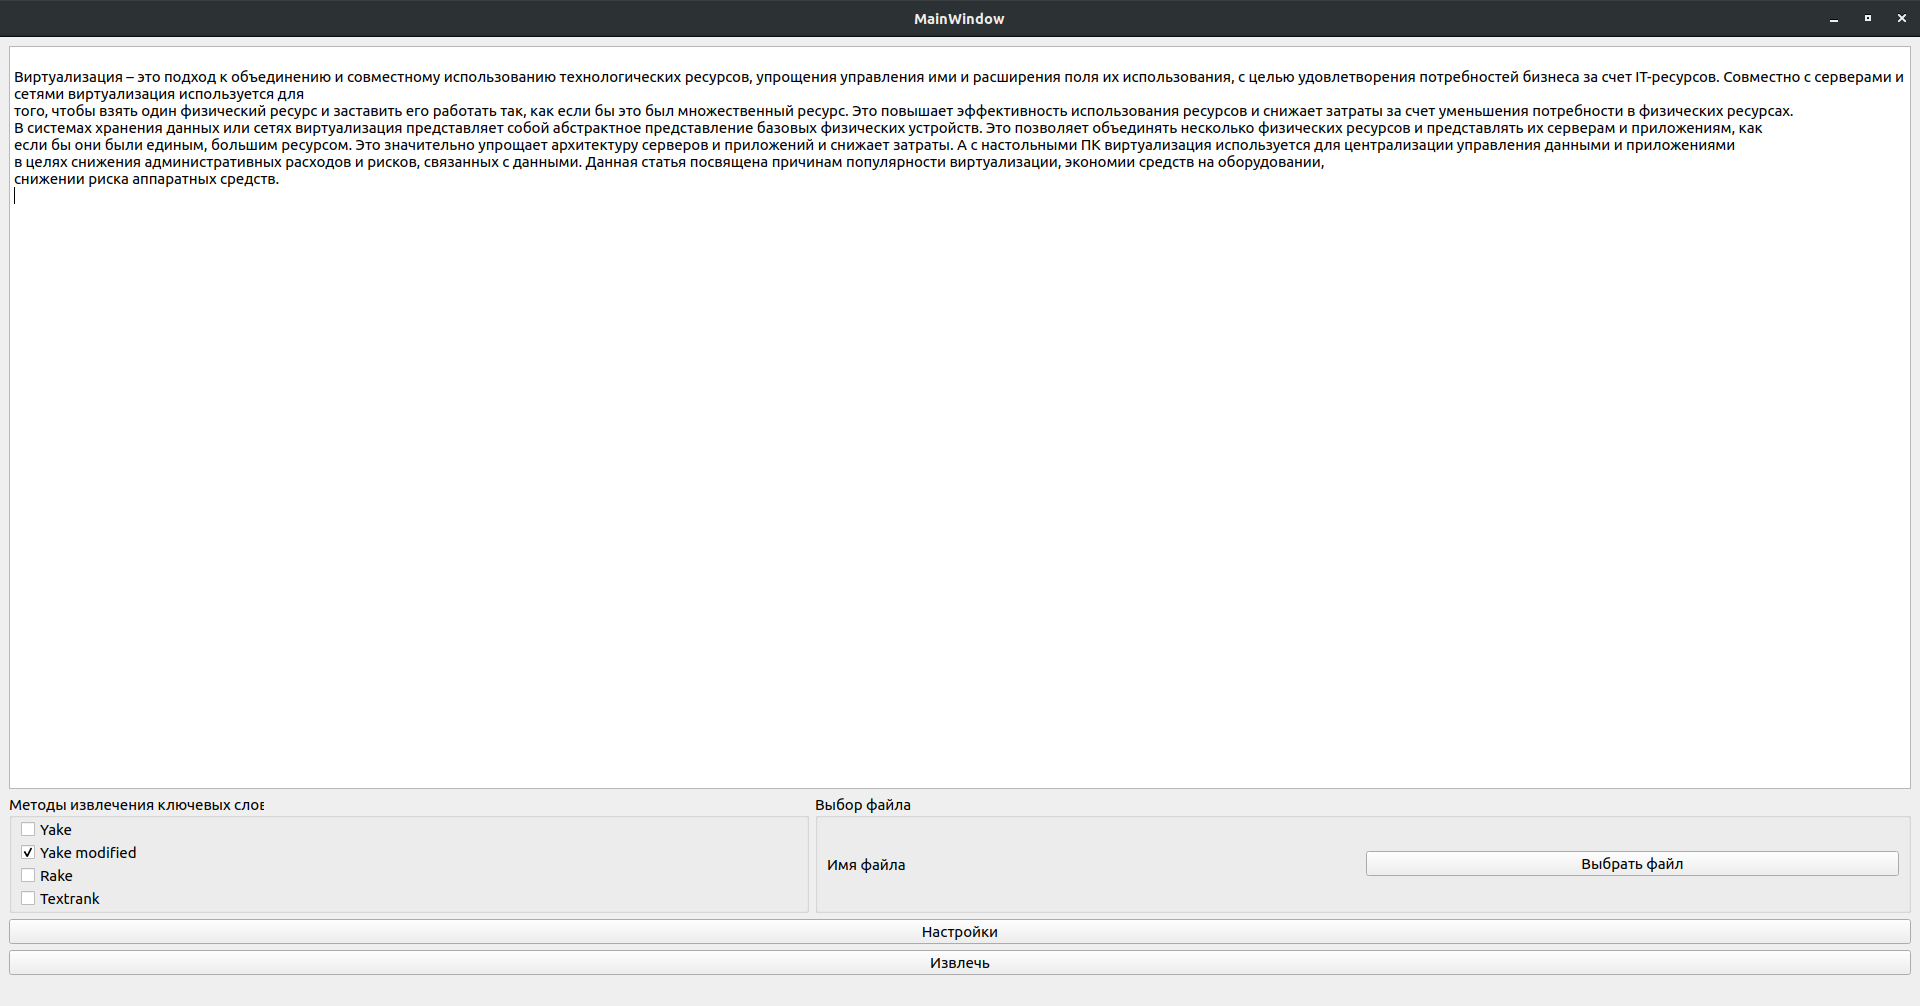
\includegraphics[width=0.7\linewidth]{src/img/tech/nbarsukov_20220605_a9ea}
	\caption{Главное окно}
	\label{fig:nbarsukov20220605a9ea}
\end{figure}


\begin{figure}[!h]
	\centering
	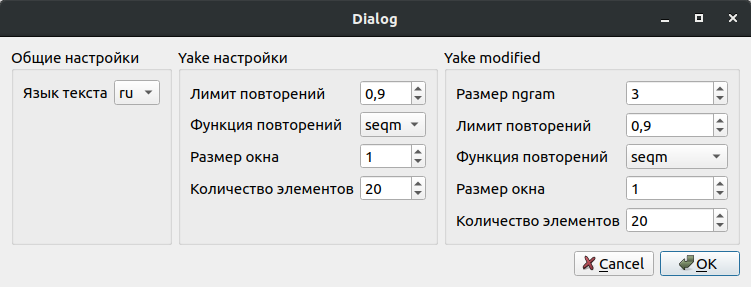
\includegraphics[width=0.7\linewidth]{src/img/programm/settings}
	\caption{Окно настроек методов}
	\label{fig:settings}
\end{figure}

% TODO: \usepackage{graphicx} required
\begin{figure}
	\centering
	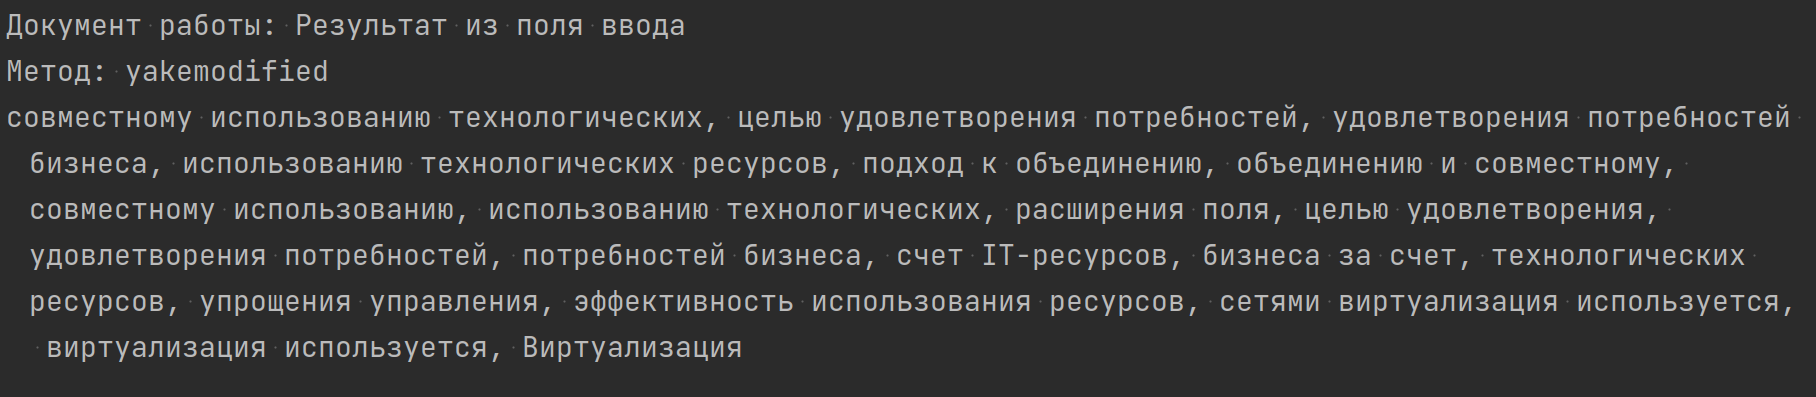
\includegraphics[width=0.7\linewidth]{src/img/tech/nbarsukov_20220605_6adf}
	\caption{Результат извлечения ключевых слов}
	\label{fig:nbarsukov202206056adf}
\end{figure}

Пользовательский интерфейс состоит из нескольких окон.
На рисунке \ref{fig:nbarsukov20220605a9ea} представлено главное окно программы.
В данном окне пользователь может указать фрагмент текста, выбрать файл формата pdf для дальнейшего извлечение текстовой информации, выбрать алгоритмы, открыть окно c параметрами методов, изображенное на рисунке \ref{fig:settings} и запустить процесс извлечения ключевых слов.

На вход ожидаются:
\begin{enumerate}
	\item параметры методов;
	\item документ формата pdf или тест
\end{enumerate}
На выходе получем список кортежей, состоящий из ключевых слов и оценок.
Результат работы алгоритма, отображен на рисунке \ref{fig:result} и представляет собой список извлеченных ключевых слов.

\section{Среда разработки}
Интегрированная среда разработки или IDE (Integrated Development Environment) - специальный программный комплекс, предназначенный для полного цикла написания и тестирования программ на определенном языке.

Интегрированная среда разработки облегчает работу, предоставляя программистам средства для разработки программного обеспечения, такие как редактор исходного кода, средства автоматизации сборки и отладчик. 
IDE облегчает визуальное представление файлов и делает его более понятным для пользователя.

Средой разработки для разработки ПО была выбрана IDE PyCharm от компании JetBrains, специализирующейся на производстве инструментов для профессиональной разработки программного обеспечения.
Данная среда была выбрана из за следующих удобств и преимуществ:
\begin{enumerate}
	\item наличие полноценного отладчика как для кода так и для тестов;
	\item встроенная подсветка синтаксиса;
	\item встроенный терминал;
	\item интеграция с системой контроля версий (VCS) git;
	\item поддержка множественных конфигураций запуска;
	\item встроенный анализатор классов;
\end{enumerate}

\section{Система контроля версий}
Во время процесса разработки мною была использованна система контроля версий Git (https://git-scm.com). 
Система контроля версий с помощью репозиториев решает проблемы с переносом программного кода на другие устройства, его резервным копированием, а так же дает возможность разделения версий продукта во время разработки, что позволяет при внесении изменений или модификациях всегда иметь рабочею версию проекта.

\section{Вывод}
В результате выполнения данного раздела был выбран язык программирования и инструменты в виде библиотек и фреймворков, необходимых для реализации разрабатываемого программного обеспечения.
Проведен детальной обзор разработанного пользовательского интерфейса с применением QT5.
Описаны входные и выходные данные разрабатываемого метода.
Обоснован выбор интегрированной среды разработки IDE и системы контроля версий VCS
